Hereafter we will limit ourselves to a system which now contains only one-particle-one-hole excitations beyond the chosen state $\ket{c}$.
Using the possible Slater determinants from exercise a) for the helium atom, find the expressions (without inserting the explicit values for the matrix elements first) for % chktex 10 % tex-fmt: skip
\begin{equation*}
    \expval{c}{\hat{H}}{\Phi_i^a},
\end{equation*}
and
\begin{equation*}
    \expval{\Phi_i^a}{\hat{H}}{\Phi_j^b}.
\end{equation*}
Represent these expressions in a diagrammatic form, both for the onebody part and the two-body part of the Hamiltonian.

Insert then the explicit values for the various matrix elements and set up the final Hamiltonian matrix and diagonalize it using for example Python as programming language.
Compare your results from those of exercise b) and comment your results. % chktex 10 % tex-fmt: skip

The exact energy with our Hamiltonian is $-2.9037$ atomic units for helium.
This value is also close to the experimental energy.

\subsection{}
In order to be able to handle the more complicated systems, we partition the Hamiltonian into
\begin{equation}
    \hat{H} = \underbrace{\mathcal{E}_0^{\text{Ref}}}_{\expval{c}{\hat{H}}{c}} + \hat{F}_N + \hat{V}_N,
\end{equation}
where
\begin{align*}
    \hat{F}_N &= \sum_{pq} \expval{p}{f}{q} \{a_p^\dagger a_q\}, \qquad
    \expval{p}{f}{q} = \expval{p}{\hat{h}_0}{q} + \sum_{i} \expval{pi}{V}{qi}_{AS}, \\
    \hat{V}_N &= \frac{1}{4} \sum_{pqrs} \expval{pq}{V}{rs}_{AS} \{a_p^\dagger a_q^\dagger a_s a_r\}.
\end{align*}

Considering then $\expval{c}{\hat{H}}{\Phi_i^a}$, we firstly have $\expval{c}{\mathcal{E}_0^{\text{Ref}}}{\Phi_i^a} = 0$, as $\braket{c}{\Phi_i^a} = 0$.
For the next term, we have
\begin{align*}
    \expval{c}{\hat{F}_N}{\Phi_i^a} &= \sum_{pq} \expval{p}{f}{q} \expval{c}{\{ a_p^\dagger a_q \}}{\Phi_i^a}
    = \sum_{pq} \expval{p}{f}{q} \wick{
        \langle c \vert
        \{ \c2 a_p^\dagger \c1 a_q \}
        \{ \c1 a_a^\dagger \c2 a_i \}
        \vert c \rangle
    } \\
    &= \sum_{pq} \expval{p}{f}{q} \delta_{pi} \delta_{qa}
    = \expval{i}{f}{a} \\
    &= \expval{i}{\hat{h}_0}{a} + \sum_{j} \expval{ij}{V}{aj}_{AS}.
\end{align*}
For the last term, we get
\begin{align*}
    \expval{c}{\hat{V}_N}{\Phi_i^a} &= \frac{1}{4} \sum_{pqrs} \expval{pq}{V}{rs}_{AS} \expval{c}{\{a_p^\dagger a_q^\dagger a_s a_r \}}{\Phi_i^a} \\
    &= \frac{1}{4} \sum_{pqrs} \expval{pq}{V}{rs}_{AS} \wick{
        \langle c \vert
        \{ a_p^\dagger a_q^\dagger a_s a_r \}
        \{ a_a^\dagger a_i \}
        \vert c \rangle
    } \\
    &= 0,
\end{align*}
which vanishes as this would require a contraction within the normal ordered operator $\{a_p^\dagger a_q^\dagger a_s a_r\}$.

Considering next $\expval{\Phi_i^a}{\hat{H}}{\Phi_{j}^{b}}$, we have
\begin{equation*}
    \expval{\Phi_i^a}{\mathcal{E}_0^{\text{Ref}}}{\Phi_{j}^{b}} = \mathcal{E}_0^{\text{Ref}}
    \expval{c}{\wick{
            \{ \c2 a_i^\dagger \c1 a_a \}
            \{ \c1 a_b^\dagger \c2 a_j \}
        }
    }{c}
    = \delta_{ij} \delta_{ab} \mathcal{E}_0^{\text{Ref}}.
\end{equation*}
Next, we have
\begin{align*}
    \expval{\Phi_i^a}{\hat{F}_N}{\Phi_{j}^{b}}
    &= \sum_{pq} \expval{p}{f}{q} \expval{\Phi_i^a}{\{ a_p^\dagger a_q \}}{\Phi_{j}^{b}} \\
    &= \sum_{pq}
    \expval{p}{f}{q}
    \expval{c}{
        \wick{
            \{ a_i^\dagger a_a \}
            \{ a_p^\dagger a_q \}
            \{ a_b^\dagger a_j \}
        }
    }{c}.
\end{align*}
Considering the contractions seperately, we have the two possible contractions
\begin{align*}
    \wick{
        \langle c \vert
        \{ \c2 a_i^\dagger \c1 a_a \}
        \{ \c1 a_p^\dagger \c1 a_q \}
        \{ \c1 a_b^\dagger \c2 a_j \}
        \vert c \rangle
    }
    &= \delta_{ij} \delta_{ap} \delta_{bq}, \\
    \wick{
        \langle c \vert
        \{ \c1 a_i^\dagger \c2 a_a \}
        \{ \c3 a_p^\dagger \c1 a_q \}
        \{ \c2 a_b^\dagger \c3 a_j \}
        \vert c \rangle
    } &= -\delta_{iq} \delta_{ab} \delta_{jp},
\end{align*}
leaving us with
\begin{equation*}
    \expval{\Phi_i^a}{\hat{F}_N}{\Phi_{j}^{b}} = \expval{a}{f}{b} \delta_{ij} - \expval{j}{f}{i} \delta_{ab}.
\end{equation*}
Finally, considering the last term, we have
\begin{align*}
    \expval{\Phi_i^a}{\hat{V}_N}{\Phi_{j}^{b}}
    &= \frac{1}{4} \sum_{pqrs} \expval{pq}{V}{rs}_{AS} \expval{\Phi_i^a}{\{a_p^\dagger a_q^\dagger a_s a_r\}}{\Phi_{j}^{b}} \\
    &= \frac{1}{4} \sum_{pqrs} \expval{pq}{V}{rs}_{AS} \expval{c}{
        \wick{
            \{ a_i^\dagger a_a \}
            \{ a_p^\dagger a_q^\dagger a_s a_r \}
            \{ a_b^\dagger a_j \}
        }
    }{c}.
\end{align*}
Considering the contractions seperately, we have the four possible contractions
\begin{align*}
    \wick{
        \langle c \vert
        \{ \c2 a_i^\dagger \c1 a_a \}
        \{ \c1 a_p^\dagger \c3 a_q^\dagger \c2 a_s \c1 a_r \}
        \{ \c1 a_b^\dagger \c3 a_j \}
        \vert c \rangle
    }
    &= -\delta_{is} \delta_{ap} \delta_{jq} \delta_{br}, \\
    \wick{
        \langle c \vert
        \{ \c2 a_i^\dagger \c1 a_a \}
        \{ \c3 a_p^\dagger \c1 a_q^\dagger \c2 a_s \c1 a_r \}
        \{ \c1 a_b^\dagger \c3 a_j \}
        \vert c \rangle
    } &= \delta_{is} \delta_{aq} \delta_{jp} \delta_{br}, \\
    \wick{
        \langle c \vert
        \{ \c2 a_i^\dagger \c1 a_a \}
        \{ \c1 a_p^\dagger \c3 a_q^\dagger \c1 a_s \c2 a_r \}
        \{ \c1 a_b^\dagger \c3 a_j \}
        \vert c \rangle
    } &= \delta_{ir} \delta_{ap} \delta_{jq} \delta_{bs}, \\
    \wick{
        \langle c \vert
        \{ \c2 a_i^\dagger \c1 a_a \}
        \{ \c3 a_p^\dagger \c1 a_q^\dagger \c1 a_s \c2 a_r \}
        \{ \c1 a_b^\dagger \c3 a_j \}
        \vert c \rangle
    } &= -\delta_{ir} \delta_{aq} \delta_{jp} \delta_{bs}.
\end{align*}
Any contraction between $\{a_i^\dagger a_a\}$ and $\{a_b^\dagger a_j\}$ will vanish, as this would require a contraction within central normal ordered operator.
This leaves us with
\begin{align*}
    \expval{\Phi_i^a}{\hat{V}_N}{\Phi_{j}^{b}}
    &= \frac{1}{4} \sum_{pqrs} \expval{pq}{V}{rs}_{AS} \\
    &\times \Big[
        - \delta_{is} \delta_{ap} \delta_{jq} \delta_{br}
        + \delta_{is} \delta_{aq} \delta_{jp} \delta_{br}
        + \delta_{ir} \delta_{ap} \delta_{jq} \delta_{bs}
        - \delta_{ir} \delta_{aq} \delta_{jp} \delta_{bs}
    \Big],
\end{align*}
which when inserted gives
\begin{align*}
    \expval{\Phi_i^a}{\hat{V}_N}{\Phi_{j}^{b}} &= \frac{1}{4} \big[
        -\expval{aj}{V}{bi}_{AS} + \expval{ja}{V}{bi}_{AS} + \expval{aj}{V}{ib}_{AS} - \expval{ja}{V}{ib}_{AS}
    \big] \\
    &= \frac{1}{4} \big[
        \expval{aj}{V}{ib}_{AS} + \expval{ja}{V}{bi}_{AS} + \expval{aj}{V}{ib}_{AS} + \expval{ja}{V}{bi}_{AS}
    \big] \\
    &= \expval{aj}{V}{ib}_{AS}.
\end{align*}
We have thus shown that
\begin{equation}
    \begin{split}
        \expval{c}{\hat{H}}{\Phi_i^a} &= \expval{i}{\hat{h}_0}{a} + \sum_{j} \expval{ij}{V}{aj}_{AS}, \\
        \expval{\Phi_i^a}{\hat{H}}{\Phi_{j}^{b}} &= \delta_{ij} \delta_{ab} \mathcal{E}_0^{\text{Ref}} + \expval{a}{f}{b} \delta_{ij} - \expval{j}{f}{i} \delta_{ab} + \expval{aj}{V}{ib}_{AS}.
    \end{split}
\end{equation}
The diagrammatic representation of these expressions are shown in Fig.~\ref{fig:ground-excited}.
\begin{figure}
    \centering
    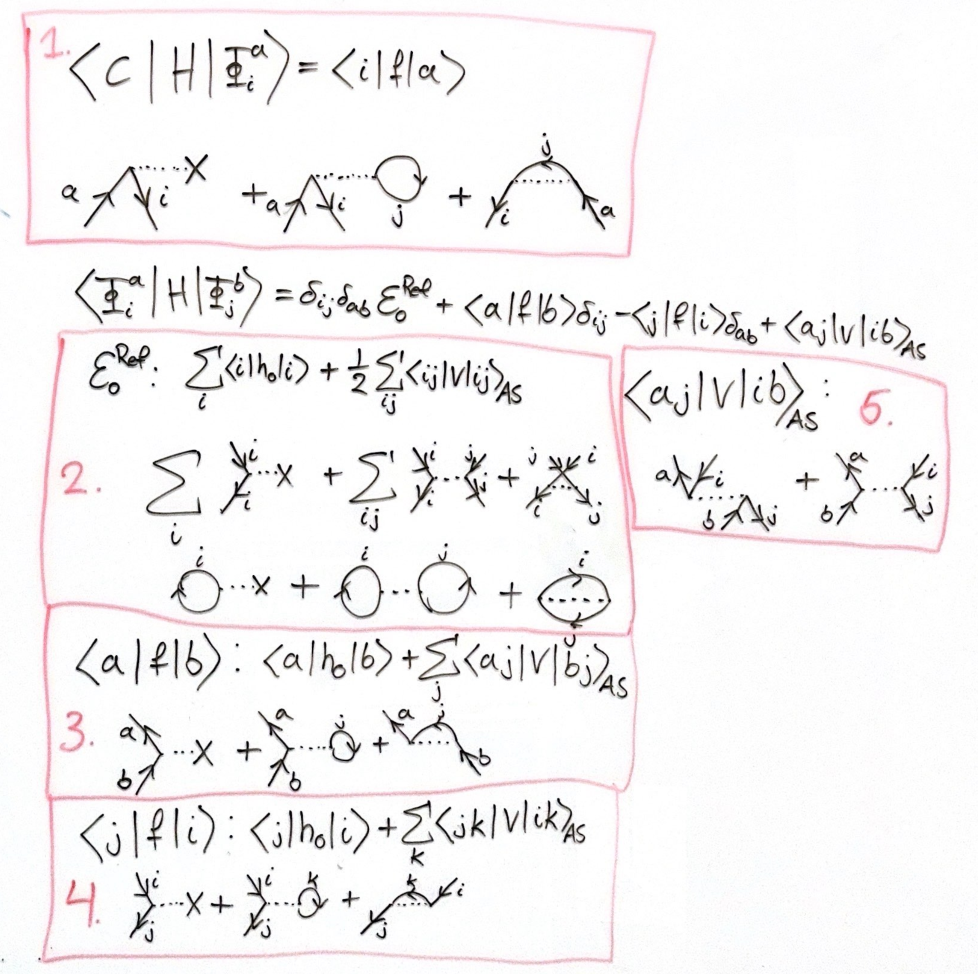
\includegraphics[width=0.8\textwidth]{figs/ground-excited.pdf}
    \caption{
        Diagrammatic representation of the one-body and two-body parts of the Hamiltonian for the ground state and an excited state.
        Box 1 contains the diagram for $\expval{c}{\hat{H}}{\Phi_i^a}$, while the sum of the remaining boxes contain the diagram for each term in the expression for $\expval{\Phi_i^a}{\hat{H}}{\Phi_{j}^{b}}$.\label{fig:ground-excited}
    }
\end{figure}

Inserting for the explicit matrix elements, we get that the energy with our Hamiltonian is $-2.8386$ atomic units, or $-77.2112 \ \text{eV}$ for the helium atom.
We see that we have a higher value than the exact energy, which is expected as the true energy serves as a lower bound to the truncated Hamiltonian.
We also see an improvement from our previous results, which stem from the fact that we are truncating at a higher level of excitations.
The energy is computed with the code in \verb|diagonalization.py|.
